% !TeX root = ../main.tex

\newlecture[Bond Price Sensitivity][Oct 5, 2026]

Bond price sensitivity is measured two ways:
\begin{itemize}
    \item \b{Yield sensitivity}: Macaulay duration, modified duration, and the connection between them.
    \item \b{Spot rate curve sensitivity}: Fisher-Weil duration and quasi-modified duration.
\end{itemize}

\b{Question}: I would like to invest in a bond, but I am worried that bond yields may change in the future. Should I invest in a short or long maturity bond to reduce the effect of yield changes on the value of my bond? Should I choose a bond with large or small coupons?
\\\b{Answer}: We need a way to compute the \dbb{sensitivity of bond prices to yield/interest}.

\header{Sensitivity Related to Time to Maturity}
\begin{center}
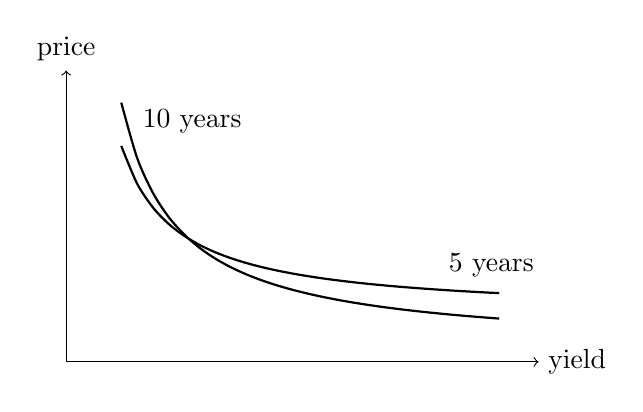
\begin{tikzpicture}
    \draw[->] (0,0) -- (6,0) node[right] {yield};
    \draw[->] (0,0) -- (0,3.7) node[above] {price};
    \draw[thick, domain=0.7:5.5, smooth, variable=\x] plot ({\x}, {0.6 + 1.5/\x});
    \draw[thick, domain=0.7:5.5, smooth, variable=\x] plot ({\x}, {0.15 + 2.2/\x});
    \node[right] at (0.85,3.05) {10 years};
    \node[above] at (5.4,0.95) {5 years};
\end{tikzpicture}
\end{center}
\keypoint{The longer the time to maturity, the more sensitive the price of the bond is to the yield.}

\header{Duration}
Maturity time is related to the sensitivity of the bond price to its yield.
\\In the case of zero-coupon bonds, the \rb{duration} (numerical measure for sensitivity) is the maturity (time measure), as the center of gravity is completely on the singular cash flow at maturity.
\\When there are coupons, the relationship is no longer direct.

\heading{Macaulay Duration}
Take the \dbb{weighted average} of the times to the cash flows, where each cash flow is weighted by its \dbb{present value} (computed with the yield) divided by the total present value.

\begin{center}
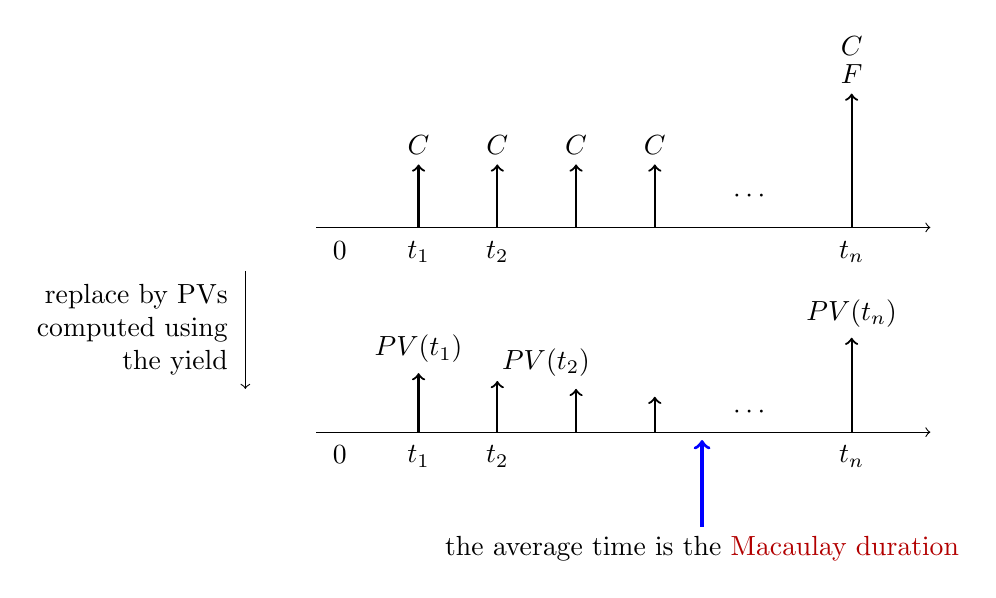
\begin{tikzpicture}
    % original cash flows
    \draw[->] (-0.3,0) -- (7.5,0);
    \node[below] at (0,-0.05) {$0$};
    \node[below] at (1,-0.05) {$t_1$};
    \node[below] at (2,-0.05) {$t_2$};
    \node[below] at (6.5,-0.05) {$t_n$};
    \foreach \x in {1,2,3,4} {
        \draw[->, thick] (\x,0) -- (\x,0.8) node[above] {$C$};
    }
    \node at (5.2,0.4) {$\cdots$};
    \draw[->, thick] (6.5,0) -- (6.5,1.7);
    \node at (6.5,2.3) {$C$};
    \node at (6.5,1.95) {$F$};
    % present values
    \begin{scope}[yshift=-2.6cm]
        \draw[->] (-0.3,0) -- (7.5,0);
        \node[below] at (0,-0.05) {$0$};
        \node[below] at (1,-0.05) {$t_1$};
        \node[below] at (2,-0.05) {$t_2$};
        \node[below] at (6.5,-0.05) {$t_n$};
        \draw[->, thick] (1,0) -- (1,0.75) node[above] {$PV(t_1)$};
        \draw[->, thick] (2,0) -- (2,0.65) node[above right=-2pt] {$PV(t_2)$};
        \draw[->, thick] (3,0) -- (3,0.55);
        \draw[->, thick] (4,0) -- (4,0.45);
        \node at (5.2,0.25) {$\cdots$};
        \draw[->, thick] (6.5,0) -- (6.5,1.2) node[above] {$PV(t_n)$};
        \draw[->, very thick, blue] (4.6,-1.2) -- (4.6,-0.1);
        \node[below, align=center] at (4.6,-1.2) {the average time is the \textcolor{red!70!black}{Macaulay duration}};
    \end{scope}
    \draw[->] (-1.2,-0.55) -- (-1.2,-2.05);
    \node[left, align=right] at (-1.3,-1.3) {replace by PVs\\computed using\\the yield};
\end{tikzpicture}
\end{center}

\begin{definition}[\rb{Macaulay Duration}]
    \[\boxed{\begin{aligned}
        D &= \frac{PV(t_1)t_1 + PV(t_2)t_2 + \cdots + PV(t_n)t_n}{PV_{total}}\\
        &= w_{t_1}t_1 + w_{t_2}t_2 + \cdots + w_{t_n}t_n\\
        &\text{where } w_{t_i} = \frac{PV(t_i)}{PV_{total}}
    \end{aligned}}\]
    Where $PV(t_i)$ is the present value of the cash flow at time $t_i$, computed \ul{using the yield as the interest rate}, and $PV_{total} = \sum_{i} PV(t_i)$ is the present value of the entire cash flow.
    \\Macaulay duration is a \dbb{weighted average of times}, so it is quoted in \dbb{years}. 
\end{definition}
\b{Economic meaning}: imagine buying a bond today. Macaulay duration answers ``if I view all future payments as one equivalent payment, at what average future date would I receive it?'' It is an \dbb{average waiting time to receiving cash}.

\heading{Macaulay Duration and Maturity}
\begin{itemize}
    \item Zero-coupon bond: Macaulay duration $=$ maturity date.
    \item Coupon bond: Macaulay duration $<$ maturity date.
\end{itemize}
\keypoint{\db{You should think}: a bond with \rb{Macaulay duration $D$} has the same yield sensitivity as a \rb{zero-coupon bond with maturity $D$}.}
Back to the opening question: to reduce the effect of yield changes, choose a bond with a \dbb{shorter maturity} and \dbb{larger coupons}, since both pull the duration down (larger coupons put more PV weight on earlier times).

\heading{Macaulay Duration Formula}
For a coupon bond:
\[\boxed{\begin{gathered}
    D = \frac{1+\frac{\lambda}{m}}{\lambda} - \frac{1 + \frac{\lambda}{m} + n\left(\frac{c}{m} - \frac{\lambda}{m}\right)}{c\left[\left(1+\frac{\lambda}{m}\right)^n - 1\right] + \lambda}\\[4pt]
    \begin{array}{@{}l@{}}
        c: \text{coupon rate per year}\\
        \lambda: \text{yield}\\
        m: \text{periods per year}\\
        n: \text{periods remaining}
    \end{array}
\end{gathered}}\]

\begin{example}
    A 2-year bond with face value \$100, a 20\% semi-annual coupon (\$10 every 6 months), and a yield of 4\% compounded semi-annually (2\% per period). Find the Macaulay duration.
    \\Total present value:
    \[PV_{total} = \sum_{i=1}^{4}\frac{10}{(1+0.02)^i} + \frac{100}{(1+0.02)^4} = 9.804 + 9.612 + 9.423 + 9.238 + 92.385 = 130.462\]
    Macaulay duration:
    \[D = \underbrace{0.5}_{t_1}\cdot\frac{9.804}{130.462} + \underbrace{1.0}_{t_2}\cdot\frac{9.612}{130.462} + \underbrace{1.5}_{t_3}\cdot\frac{9.423}{130.462} + \underbrace{2.0}_{t_4}\cdot\frac{9.238 + 92.385}{130.462} = 1.777 \text{ years}\]
    \begin{center}
    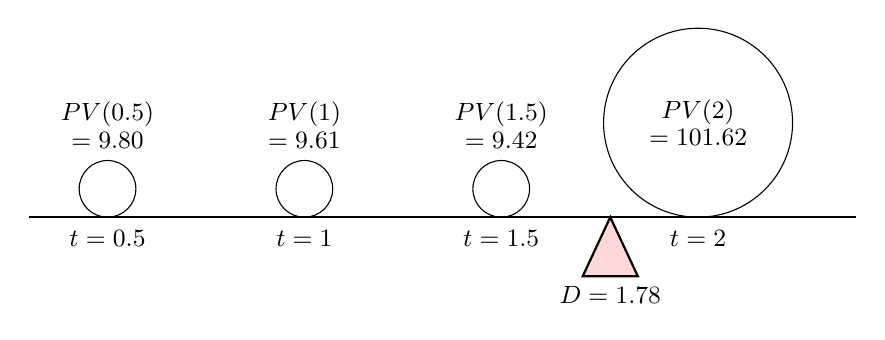
\begin{tikzpicture}[x=5cm]
        % beam
        \draw[thick] (0.3,0) -- (2.4,0);
        % weights: bigger PV = bigger circle
        \foreach \t/\pv in {0.5/9.80, 1/9.61, 1.5/9.42} {
            \draw (\t,0.36) circle (0.36cm);
            \node[above, align=center] at (\t,0.75) {\small $PV(\t)$\\[-2pt]\small $= \pv$};
            \node[below] at (\t,-0.05) {\small $t = \t$};
        }
        \draw (2,1.2) circle (1.2cm);
        \node[align=center] at (2,1.2) {\small $PV(2)$\\[-2pt]\small $= 101.62$};
        \node[below] at (2,-0.05) {\small $t = 2$};
        % fulcrum at the Macaulay duration
        \draw[thick, fill=red!15] (1.777,0) -- (1.707,-0.75) -- (1.847,-0.75) -- cycle;
        \node[below] at (1.777,-0.75) {\small $D = 1.78$};
    \end{tikzpicture}
    \end{center}
    Think of the PVs as weights on a seesaw over the timeline: the "balance point" is at $t = 1.78$, pulled close to $t = 2$ by the large final payment ($PV(2) = 101.62$). The formula above gives the same answer with $c = 0.2$, $\lambda = 0.04$, $m = 2$, $n = 4$.
    \\(Equivalently, the yield is $2\ln(1.02) = 3.9605\%$ continuously compounded.)
\end{example}

\heading{Modified Duration}
Why not calculate the sensitivity of a bond to the yield exactly?
\begin{definition}[\rb{Modified Duration}]
    Let $P$ be the price of a bond. The modified duration $D_m$ of the bond is
    \[\boxed{\begin{gathered}
        D_m = -\frac{1}{P(\lambda_0)}\left.\frac{dP(\lambda)}{d\lambda}\right|_{\lambda = \lambda_0}\\[4pt]
        \begin{aligned}
            \lambda_0 &: \text{the current yield}\\
            P(\lambda_0) &: \text{the current price of the bond}
        \end{aligned}
    \end{gathered}}\]
\end{definition}
\begin{itemize}
    \item Roughly, think \dbb{sensitivity = derivative}.
    \item The minus sign is so it won't be a negative quantity (price falls as yield rises).
    \item Dividing by $P$ makes it a \dbb{relative} sensitivity.
\end{itemize}

Modified duration gives the \ul{percentage change in price for a change in yield}:
\[D_m \approx -\frac{1}{P}\frac{\Delta P}{\Delta\lambda} \quad \Rightarrow \quad \boxed{\Delta P \approx -D_m P \Delta\lambda}\]

\begin{example}
    If the yield increases by 1\%, a bond with modified duration 5 drops in price by about 5\%.
    \\With a current price of \$100.
    \[\Delta P \approx -D_m P\Delta\lambda = -5(\$100)(0.01) = -\$5\]
\end{example}

\heading{Relationship between Modified and Macaulay Duration}
\[\boxed{\begin{gathered}
    D_m = \frac{D}{1+\frac{\lambda}{m}}\\[4pt]
    \begin{array}{@{}l@{}}
        D_m: \text{modified duration}\\
        D: \text{Macaulay duration}\\
        \lambda: \text{yield}\\
        m: \text{number of compounding periods per year}
    \end{array}
\end{gathered}}\]
\begin{enumerate}[label=(\roman*)]
    \item They differ only by a \dbb{constant factor}.
    \item With continuous compounding ($m\to\infty$), $D_m \to D$.
\end{enumerate}

\begin{proof}
    \b{Setup.} Suppose there are $m$ periods per year, the yield is $\lambda$, and the bond pays cash flow $c_k$ at period $k$ (time $k/m$ years), for $k = 0, 1, \dots, n$. Then
    \[PV_k = \frac{c_k}{\left(1+\frac{\lambda}{m}\right)^k}, \qquad \underset{\mathclap{\substack{\Big\uparrow\\\text{Current price of bond}}}}{PV_{tot}} = \sum_{k=0}^{n}PV_k = \sum_{k=0}^{n}\frac{c_k}{\left(1+\frac{\lambda}{m}\right)^k}\]
    and the two quantities we want to relate are
    \[D = \sum_{k=0}^{n}\frac{k}{m}\frac{PV_k}{PV_{tot}} \quad \text{(Macaulay)}, \qquad D_m = -\frac{1}{PV_{tot}}\frac{dPV_{tot}}{d\lambda} \quad \text{(modified)}\]

    \b{Step 1: differentiate the price.} Only $\left(1+\frac{\lambda}{m}\right)^{-k}$ depends on $\lambda$; by the chain rule,
    \[\frac{d}{d\lambda}\left(1+\frac{\lambda}{m}\right)^{-k} = -k\left(1+\frac{\lambda}{m}\right)^{-k-1}\cdot\frac{1}{m}\]
    so differentiating $PV_{tot}$ term by term gives
    \[\frac{dPV_{tot}}{d\lambda} = -\sum_{k=0}^{n}\frac{k}{m}\frac{c_k}{\left(1+\frac{\lambda}{m}\right)^{k+1}}\]

    \b{Step 2: rewrite in terms of $PV_k$.} Pull one factor of $\left(1+\frac{\lambda}{m}\right)$ out of each denominator:
    \[\frac{dPV_{tot}}{d\lambda} = -\frac{1}{1+\frac{\lambda}{m}}\sum_{k=0}^{n}\frac{k}{m}\underbrace{\frac{c_k}{\left(1+\frac{\lambda}{m}\right)^{k}}}_{PV_k} = -\frac{1}{1+\frac{\lambda}{m}}\sum_{k=0}^{n}\frac{k}{m}PV_k\]

    \b{Step 3: plug into the definition of $D_m$.}
    \begin{align*}
        D_m &= -\frac{1}{PV_{tot}}\frac{dPV_{tot}}{d\lambda}\\
        &= -\frac{1}{PV_{tot}}\left(-\frac{1}{1+\frac{\lambda}{m}}\sum_{k=0}^{n}\frac{k}{m}PV_k\right)\\
        &= \frac{1}{1+\frac{\lambda}{m}}\underbrace{\sum_{k=0}^{n}\frac{k}{m}\frac{PV_k}{PV_{tot}}}_{D}\\
        &= \frac{D}{1+\frac{\lambda}{m}}
    \end{align*}
\end{proof}
\rb{EXAM NOTE!} remember how to calculate the \rb{DERIVATIVE! } $\boxed{\left.\frac{dP(\lambda)}{d\lambda}\right|_{\lambda = \lambda_0}}$

\begin{example}
    A 10\%, 30-year bond priced at \$100 has Macaulay duration $D = 9.94$, with semi-annual coupons.
    \begin{enumerate}[label=(\alph*)]
        \item Modified duration, and the effect of a 1\% yield increase: since the price is \$100 (par), the yield is $\lambda = 10\%$, so
        \[D_m = \frac{D}{1+\frac{\lambda}{2}} = \frac{9.94}{1.05} = 9.47\]
        A 1\% increase in yield causes about a 9.47\% drop in price.
        \item Estimated price if the yield moves to 11\%:
        \[\Delta P \approx -D_m P\Delta\lambda = -9.47(100)(0.01) = -9.47 \quad \Rightarrow \quad P \approx \$100 - \$9.47 = \$90.53\]
    \end{enumerate}
\end{example}

\header{Duration with Spot Rates}
This time we compute sensitivity to changes in the \dbb{term structure} rather than the yield. It is again basically the derivative of the bond price with respect to interest rates, properly normalized, but now we \ul{perturb the entire spot rate curve}.

\heading{Sensitivity to Spot Rates}
Assume continuous compounding. What is the sensitivity of the present value of the cash flow $(x_{t_0}, x_{t_1}, \dots, x_{t_n})$ to \dbb{parallel shifts} in the spot rate curve?
\\Note that its assumed \underline{all spot rates change at the same rate}, hence parallel shift in the curve.

\begin{center}
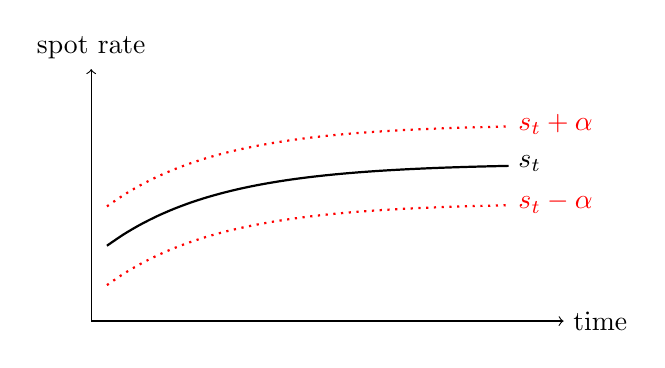
\begin{tikzpicture}
    \draw[->] (0,0) -- (6,0) node[right] {time};
    \draw[->] (0,0) -- (0,3.2) node[above] {spot rate};
    \draw[thick, domain=0.2:5.3, smooth, variable=\x] plot ({\x}, {2.0 - 1.2*exp(-0.7*\x)});
    \draw[thick, dotted, red, domain=0.2:5.3, smooth, variable=\x] plot ({\x}, {2.5 - 1.2*exp(-0.7*\x)});
    \draw[thick, dotted, red, domain=0.2:5.3, smooth, variable=\x] plot ({\x}, {1.5 - 1.2*exp(-0.7*\x)});
    \node[right] at (5.3,2.0) {$s_t$};
    \node[right, red] at (5.3,2.5) {$s_t + \alpha$};
    \node[right, red] at (5.3,1.5) {$s_t - \alpha$};
\end{tikzpicture}
\end{center}

Shift the whole curve by $\alpha$:
\[PV = \sum_{i=0}^{n}x_{t_i}e^{-s_{t_i}t_i} \quad \rightarrow \quad PV(\alpha) = \sum_{i=0}^{n}x_{t_i}e^{-(s_{t_i}+\alpha)t_i}\]
To determine sensitivity, \b{take the derivative with respect to $\alpha$ and evaluate at $\alpha = 0$}. Note that the current present value is $PV(0)$.

\begin{definition}[\rb{Duration with respect to Spot Rates}]
    \[\boxed{D(s_t) = \underset{\substack{\left\uparrow\vphantom{\rule{0pt}{6.5ex}}\right.\\\mathrlap{\hspace{-1.3cm}\text{price falls as rates rise } \left(\frac{dPV}{d\alpha} < 0\right)\text{,}}\\\mathrlap{\hspace{-1.3cm}\text{so the minus makes } D(s_t) > 0}}}{-}\Bigg(\underset{\mathclap{\substack{\Big\uparrow\\\text{current price}}}}{\frac{1}{PV(0)}}\Bigg)\underset{\mathclap{\substack{\Bigg\uparrow\\\text{shift curve by } \alpha}}}{\left.\frac{dPV(\alpha)}{d\alpha}\right|_{\alpha = 0}}}\]
    This is the \dbb{same recipe as modified duration}; only the thing we perturb changes:
    \[\underbrace{D_m = -\frac{1}{P(\lambda_0)}\left.\frac{dP(\lambda)}{d\lambda}\right|_{\lambda = \lambda_0}}_{\text{perturb the yield } \lambda} \qquad\longleftrightarrow\qquad \underbrace{D(s_t) = -\frac{1}{PV(0)}\left.\frac{dPV(\alpha)}{d\alpha}\right|_{\alpha = 0}}_{\text{perturb every spot rate by } \alpha}\]
    \begin{itemize}
        \item With \dbb{continuous compounding}, it is called the \rb{Fisher-Weil duration} (it looks similar to Macaulay!):
        \[\boxed{D_{FW} = \left(\frac{1}{PV}\right)\sum_{i=0}^{n}\underset{\mathclap{\substack{\Big\uparrow\\\text{time}}}}{t_i}\underbrace{x_{t_i}e^{-s_{t_i}t_i}}_{PV_{t_i}}}\]
        since $\left.\frac{dPV(\alpha)}{d\alpha}\right|_{\alpha=0} = -\sum_{i=0}^{n}t_i x_{t_i}e^{-s_{t_i}t_i}$.
        \\It is the same as the Macaulay duration, but generalized for all cash flow vectors, while Macaulay is for bonds.
        \\If the spot curve is flat ($s_{t_i} = \lambda$ for all $i$), then $D_{FW} = D$.
        \item With \dbb{discrete compounding} ($m$ periods per year, $s_i$ the spot rate for period $i$), it is called the \rb{quasi-modified duration}:
        \\Note it is not the Macaulay duration, as there is a factor of $+1$ in the power of the denominator.
        \\If the spot curve is flat ($s_i = \lambda$ for all $i$), then $D_Q = \frac{D}{1+\frac{\lambda}{m}} = D_m$.
    \end{itemize}
\end{definition}

\heading{Simplification for Continuous Compounding Only!}
Under continuous compounding, all the duration formulas look like a \dbb{weighted average of times}:
\[D_{FW} = \sum_{i=0}^{n}t_i\frac{PV_{t_i}}{PV_{Total}}\]
The only difference is the rate used to compute the PVs:
\begin{itemize}
    \item Macaulay and modified duration use the \dbb{yield}: $PV_{t_i} = x_{t_i}e^{-\lambda t_i}$
    \item Fisher-Weil duration uses the \dbb{spot rates}: $PV_{t_i} = x_{t_i}e^{-s_{t_i}t_i}$
\end{itemize}

\begin{example}
    \begin{center}
    \begin{tikzpicture}
        \draw[->] (0,0) -- (6,0) node[right] {time};
        \draw[->] (0,0) -- (0,2.8) node[above] {spot rate};
        \draw[thick, domain=0.2:5.3, smooth, variable=\x] plot ({\x}, {2.2 - 1.2*exp(-0.7*\x)});
        \draw[thick, dotted, red, domain=0.2:5.3, smooth, variable=\x] plot ({\x}, {1.7 - 1.2*exp(-0.7*\x)});
        \node[right] at (5.3,2.2) {$s_t$};
        \node[right, red] at (5.3,1.7) {$s_t - 2\%$};
    \end{tikzpicture}
    \end{center}
    The entire spot rate curve drops by 2\%. A bond with Fisher-Weil duration 10 changes in price by approximately $-D_{FW}\Delta\alpha = -10(-0.02) = +20\%$, i.e.\ it \dbb{increases by 20\%}.
\end{example}

\header{Summary}
\begin{framed}
    \b{Macaulay duration} is a weighted average of the times to cash flows:
    \[D = w_{t_1}t_1 + w_{t_2}t_2 + \cdots + w_{t_n}t_n, \qquad w_{t_i} = \frac{PV(t_i)}{PV_{total}}\]
    The other durations measure a percentage change in price for a change in either the yield or a parallel shift of the spot rate curve.
    \begin{itemize}
        \item \b{Modified duration} uses the yield, and is related to Macaulay duration by
        \[D_m = -\frac{1}{P(\lambda_0)}\left.\frac{dP(\lambda)}{d\lambda}\right|_{\lambda=\lambda_0}, \qquad D_m = \frac{D}{1+\frac{\lambda}{m}}\]
        \item \b{Fisher-Weil} (continuous compounding) and \b{quasi-modified} (discrete compounding) use the spot rate curve:
        \[D(s_t) = -\left(\frac{1}{PV(0)}\right)\left.\frac{dPV(\alpha)}{d\alpha}\right|_{\alpha=0}\]
        \[D_{FW} = \left(\frac{1}{PV}\right)\sum_{i=0}^{n}t_i x_{t_i}e^{-s_{t_i}t_i}, \qquad D_Q = \left(\frac{1}{PV}\right)\sum_{i=1}^{n}\frac{\frac{i}{m}x_i}{\left(1+\frac{s_i}{m}\right)^{i+1}}\]
    \end{itemize}
\end{framed}
